%% LyX 2.2.2 created this file.  For more info, see http://www.lyx.org/.
%% Do not edit unless you really know what you are doing.
\documentclass[ruled]{article}
\usepackage{courier}
\usepackage[latin9]{inputenc}
\usepackage[letterpaper]{geometry}
\geometry{verbose}
\usepackage{color}
\usepackage{url}
\usepackage{algorithm2e}
\usepackage{amsmath}
\usepackage[unicode=true,
 bookmarks=false,
 breaklinks=false,pdfborder={0 0 1},backref=section,colorlinks=true]
 {hyperref}

\makeatletter

%%%%%%%%%%%%%%%%%%%%%%%%%%%%%% LyX specific LaTeX commands.
\providecommand{\LyX}{\texorpdfstring%
  {L\kern-.1667em\lower.25em\hbox{Y}\kern-.125emX\@}
  {LyX}}
%% Because html converters don't know tabularnewline
\providecommand{\tabularnewline}{\\}

%%%%%%%%%%%%%%%%%%%%%%%%%%%%%% Textclass specific LaTeX commands.
\newenvironment{lyxcode}
{\par\begin{list}{}{
\setlength{\rightmargin}{\leftmargin}
\setlength{\listparindent}{0pt}% needed for AMS classes
\raggedright
\setlength{\itemsep}{0pt}
\setlength{\parsep}{0pt}
\normalfont\ttfamily}%
 \item[]}
{\end{list}}

%%%%%%%%%%%%%%%%%%%%%%%%%%%%%% User specified LaTeX commands.
\title{DS-GA 1003: Machine Learning and Computational Statistics\\
Homework 3: SVM and Sentiment Analysis}  

\usepackage{amsfonts}\usepackage{capt-of}
%\usepackage{url}
\usepackage{graphicx}
\usepackage{color}
\usepackage{bbm}
\usepackage{enumerate}
\newcommand{\carlos}[1]{\textcolor{red}{Carlos: #1}}
\newcommand{\field}[1]{\mathbb{#1}} 
\newcommand{\hide}[1]{#1}
\newcommand{\pd}[2]{\frac{\partial #1}{\partial #2}}
\providecommand{\m}[1]{\mathbf{#1}}
\providecommand{\norm}[1]{\left\|#1\right\|}
\providecommand{\sign}[1]{\text{sign}\left(#1\right)}
\DeclareMathOperator*{\argmin}{arg\,min}
\providecommand{\what}{\m{\hat{w}}}
\providecommand{\dw}{\Delta w}
\providecommand{\dmw}{\Delta \m{w}}
\providecommand{\hy}{\hat{y}}


\definecolor{keywords}{RGB}{255,0,90}
\definecolor{comments}{RGB}{0,0,113}
\definecolor{red}{RGB}{160,0,0}
\definecolor{green}{RGB}{0,150,0}

\makeatother

\usepackage{listings}
\lstset{language=Python,
basicstyle={\ttfamily\small},
keywordstyle={\bfseries\color{green}},
commentstyle={\color{blue}},
stringstyle={\color{red}},
showstringspaces=false,
identifierstyle={\color{black}},
frame=tb,
showstringspaces=false,
morekeywords={include, printf}}
\begin{document}


\global\long\def\reals{\mathbf{R}}
 \global\long\def\integers{\mathbf{Z}}
\global\long\def\naturals{\mathbf{N}}
 \global\long\def\rationals{\mathbf{Q}}
\global\long\def\ca{\mathcal{A}}
\global\long\def\cb{\mathcal{B}}
 \global\long\def\cc{\mathcal{C}}
 \global\long\def\cd{\mathcal{D}}
\global\long\def\ce{\mathcal{E}}
\global\long\def\cf{\mathcal{F}}
\global\long\def\cg{\mathcal{G}}
\global\long\def\ch{\mathcal{H}}
\global\long\def\ci{\mathcal{I}}
\global\long\def\cj{\mathcal{J}}
\global\long\def\ck{\mathcal{K}}
\global\long\def\cl{\mathcal{L}}
\global\long\def\cm{\mathcal{M}}
\global\long\def\cn{\mathcal{N}}
\global\long\def\co{\mathcal{O}}
\global\long\def\cp{\mathcal{P}}
\global\long\def\cq{\mathcal{Q}}
\global\long\def\calr{\mathcal{R}}
\global\long\def\cs{\mathcal{S}}
\global\long\def\ct{\mathcal{T}}
\global\long\def\cu{\mathcal{U}}
\global\long\def\cv{\mathcal{V}}
\global\long\def\cw{\mathcal{W}}
\global\long\def\cx{\mathcal{X}}
\global\long\def\cy{\mathcal{Y}}
\global\long\def\cz{\mathcal{Z}}
\global\long\def\ind#1{1(#1)}
\global\long\def\pr{\mathbb{P}}
\global\long\def\predsp{\cy}
\global\long\def\outsp{\cy}
\global\long\def\prxy{P_{\cx\times\cy}}
\global\long\def\prx{P_{\cx}}
\global\long\def\prygivenx{P_{\cy\mid\cx}}
\global\long\def\ex{\mathbb{E}}
\global\long\def\var{\textrm{Var}}
\global\long\def\cov{\textrm{Cov}}
\global\long\def\sgn{\textrm{sgn}}
\global\long\def\sign{\textrm{sign}}
\global\long\def\kl{\textrm{KL}}
\global\long\def\law{\mathcal{L}}
\global\long\def\eps{\varepsilon}
\global\long\def\as{\textrm{ a.s.}}
\global\long\def\io{\textrm{ i.o.}}
\global\long\def\ev{\textrm{ ev.}}
\global\long\def\convd{\stackrel{d}{\to}}
\global\long\def\eqd{\stackrel{d}{=}}
\global\long\def\del{\nabla}
\global\long\def\loss{\ell}
\global\long\def\risk{R}
\global\long\def\emprisk{\hat{R}_{\ell}}
\global\long\def\lossfnl{L}
\global\long\def\emplossfnl{\hat{L}}
\global\long\def\empminimizer#1{\hat{#1}_{\ell}}
\global\long\def\minimizer#1{#1_{*}}
\global\long\def\etal{\textrm{et. al.}}
\global\long\def\tr{\operatorname{tr}}
\global\long\def\trace{\operatorname{trace}}
\global\long\def\diag{\text{diag}}
\global\long\def\rank{\text{rank}}
\global\long\def\linspan{\text{span}}
\global\long\def\proj{\text{Proj}}
\global\long\def\argmax{\operatornamewithlimits{arg\, max}}
\global\long\def\argmin{\operatornamewithlimits{arg\, min}}
\global\long\def\bfx{\mathbf{x}}
\global\long\def\bfy{\mathbf{y}}
\global\long\def\bfl{\mathbf{\lambda}}
\global\long\def\bfm{\mathbf{\mu}}
\global\long\def\calL{\mathcal{L}}
\global\long\def\vw{\boldsymbol{w}}
\global\long\def\vx{\boldsymbol{x}}
\global\long\def\vxi{\boldsymbol{\xi}}
\global\long\def\valpha{\boldsymbol{\alpha}}
\global\long\def\vbeta{\boldsymbol{\beta}}
\global\long\def\vsigma{\boldsymbol{\sigma}}
\global\long\def\vmu{\boldsymbol{\mu}}
\global\long\def\vtheta{\boldsymbol{\theta}}
\global\long\def\vd{\boldsymbol{d}}
\global\long\def\vs{\boldsymbol{s}}
\global\long\def\vt{\boldsymbol{t}}
\global\long\def\vh{\boldsymbol{h}}
\global\long\def\ve{\boldsymbol{e}}
\global\long\def\vf{\boldsymbol{f}}
\global\long\def\vg{\boldsymbol{g}}
\global\long\def\vz{\boldsymbol{z}}
\global\long\def\vk{\boldsymbol{k}}
\global\long\def\va{\boldsymbol{a}}
\global\long\def\vb{\boldsymbol{b}}
\global\long\def\vv{\boldsymbol{v}}
\global\long\def\vy{\boldsymbol{y}}
\global\long\def\hil{\ch}
\global\long\def\rkhs{\hil}
\maketitle

\textbf{Yidi Zhang}

\textbf{Instructions}: Your answers to the questions below, including
plots and mathematical work, should be submitted as a single PDF file.
It's preferred that you write your answers using software that typesets
mathematics (e.g. \LaTeX{}, \LyX{}, or MathJax via iPython), though
if you need to you may scan handwritten work. You may find the \href{https://github.com/gpoore/minted}{minted}
package convenient for including source code in your \LaTeX{} document.

\section{Introduction}

In this assignment, we'll be working with natural language data. In
particular, we'll be doing sentiment analysis on movie reviews. This
problem will give you the opportunity to try your hand at feature
engineering, which is one of the most important parts of many data
science problems. From a technical standpoint, this homework has two
new pieces. First, you'll be implementing Pegasos. Pegasos is essentially
stochastic subgradient descent for the SVM with a particular schedule
for the step-size. Second, because in natural langauge domains we
typically have huge feature spaces, we work with sparse representations
of feature vectors, where only the non-zero entries are explicitly
recorded. This will require coding your gradient and SGD code using
hash tables (dictionaries in Python), rather than numpy arrays. We
begin with some practice with subgradients and an easy problem that
introduces the Perceptron algorithm.

\section{Calculating Subgradients}

Recall that a vector $g\in\reals^{d}$ is a \textbf{subgradient} of
$f:\reals^{d}\to\reals$ at $x$ if for all $z$, 
\[
f(z)\ge f(x)+g^{T}(z-x).
\]
As we noted in lecture, there may be $0$, $1$, or infinitely many
subgradients at any point. The \textbf{subdifferential} of $f$ at
a point $x$, denoted $\partial f(x)$, is the set of all subgradients
of $f$ at $x$. 

Just as there is a calculus for gradients, there is a calculus for
subgradients\footnote{A good reference for subgradients are the \href{https://stanford.edu/class/ee364b/lectures/subgradients_notes.pdf}{course notes on Subgradients by Boyd et al}.}.
For our purposes, we can usually get by using the definition of subgradient
directly. However, in the first problem below we derive a property
that will make our life easier for finding a subgradient of the hinge
loss and perceptron loss. 
\begin{enumerate}

\pagebreak
\item {[}Subgradients for pointwise maximum of functions{]} Suppose $f_{1},\ldots,f_{m}:\reals^{d}\to\reals$
are convex functions, and 
\[
f(x)=\max_{i=1,\ldots,,m}f_{i}(x).
\]
Let $k$ be any index for which $f_{k}(x)=f(x)$, and choose $g\in\partial f_{k}(x)$.
{[}We are using the fact that a convex function on $\reals^{d}$ has
a non-empty subdifferential at all points.{]} Show that $g\in\partial f(x)$.\\%%%%%%%%%%%%2.1%%%%%%%%%%%

{\bfseries Answer 2.1:}%2.1

For $\forall a \in R^{d}$
$$f(a) = max f_{i}(x) \geq f_{k}(a) \geq f_{k} + g^{T}(a-x) =f(x) + g^{T}(a-x) $$
Thus we can get $f(a) \geq f(x) + g^{T}(a-x)$, for $\forall a \in R^{d}$. So we can conclude that $g\in\partial f(x)$.

\pagebreak
\item {[}Subgradient of hinge loss for linear prediction{]} Give a subgradient
of
\[
J(w)=\max\left\{ 0,1-yw^{T}x\right\} .
\]%%%%%%%%%%%%%%%%%%%%2.2%%%%%%%%%%%%%%%%%%%%%%%%%%
 
{\bfseries Answer 2.2:}%2.1

Suppose $g(w) = w^{T}x$, and $f(z) = max\{0, 1-yz\}$.

Using the chain rule, we get:
\begin{eqnarray*}
\frac{\partial f(g(w))}{\partial w_{i}} & = & \frac{\partial f}{\partial z}\frac{\partial g}{\partial w_{i}}
\end{eqnarray*}

\begin{eqnarray*}
g^{'}(w) &=& \begin{cases}
-y & w^{T}x<1\\
0 & otherwise
\end{cases}\\
\end{eqnarray*}
Thus we can get
\begin{eqnarray*}
\frac{\partial f(g(w))}{\partial w_{i}} &=& \begin{cases}
-yx_{i} & w^{T}x<1\\
0 & otherwise
\end{cases}\\
\frac{\partial J(w)}{\partial w} & = & \sum_{i}\frac{\partial J(w)}{\partial w_{i}}\\
& = & \sum_{i}\frac{\partial f(g(w))}{\partial w_{i}}
\end{eqnarray*}
 
\end{enumerate}

\pagebreak
\section{Perceptron}

The perceptron algorithm is often the first classification algorithm
taught in machine learning classes. Suppose we have a labeled training
set $\left(x_{1},y_{1}\right),\ldots,(x_{n},y_{n})\in\reals^{d}\times\left\{ -1,1\right\} $.
In the perceptron algorithm, we are looking for a hyperplane that
perfectly separates the classes. That is, we're looking for $w\in\reals^{d}$
such that
\[
y_{i}w^{T}x_{i}>0\;\forall i\in\left\{ 1,\ldots,n\right\} .
\]
Visually, this would mean that all the $x$'s with label $y=1$ are
on one side of the hyperplane $\left\{ x\mid w^{T}x=0\right\} $,
and all the $x's$ with label $y=-1$ are on the other side. When
such a hyperplane exists, we say that the data are \textbf{linearly
separable}. The perceptron algorithm is given in Algorithm \ref{alg:Perceptron-Algorithm}.

\begin{algorithm}[h]
\caption{\label{alg:Perceptron-Algorithm}Perceptron Algorithm}

\begin{lyxcode}
input:~Training~set~$\left(x_{1},y_{1}\right),\ldots,(x_{n},y_{n})\in\reals^{d}\times\left\{ -1,1\right\} $~\\
$w^{(0)}=\left(0,\ldots,0\right)\in\reals^{d}$~\\
$k=0$~\#~step~number~\\
repeat~\\
~~all\_correct~=~TRUE~\\
~~for~$i=1,2,\ldots,n$~\#~loop~through~data~\\
~~~~if~($y_{i}x_{i}^{T}w^{(k)}\le0$)~\\
~~~~~~$w^{(k+1)}=w^{(k)}+y_{i}x_{i}$~\\
~~~~~~all\_correct~=~FALSE~\\
~~~~else~\\
~~~~~~$w^{(k+1)}=w^{(k)}$~\\
~~~~end~if~\\
~~~~$k=k+1$~\\
~~end~for~\\
until~(all\_correct~==~TRUE)~\\
return~$w^{(k)}$~\\
\end{lyxcode}
\end{algorithm}

There is also something called the \textbf{perceptron loss,} given
by 
\[
\ell(\hat{y},y)=\max\left\{ 0,-\hat{y}y\right\} .
\]
In this problem we will see why this loss function has this name.%%%%%%%%%%%%%3%%%%%%%%%%%%%%%%
\begin{enumerate}
\item Show that if $\left\{ x\mid w^{T}x=0\right\} $ is a separating hyperplane
for a training set $\cd=\left(\left(x_{1},y_{1}\right),\ldots,(x_{n},y_{n})\right)$,
then the average perceptron loss on $\cd$ is $0$.\\%%%%%%%%%%%3.1%%%%%%%%%%%%%%%%%%%%%%%%

{\bfseries Answer 3.1:}%3.1

if $\left\{ x\mid w^{T}x=0\right\}$ is a separating hyperplane, for $\forall i$, $max(0, -y_{i}w^{T}x_{i}) = 0$.

Thus we can conclude that $\ell(\hat{y},y)=\frac{1}{n}\sum^{n}_{i=1}\max\left\{ 0,-\hat{y_{i}}y_{i}\right\}=0 $.

\pagebreak
\item Let $\ch$ be the linear hypothesis space consisting of functions
$x\mapsto w^{T}x$. Consider running stochastic subgradient descent
(SSGD) to minimize the empirical risk with the perceptron loss. We'll
use the version of SSGD in which we cycle through the data points
in each epoch. Show that if we use a fixed step size $1$, we terminate
when our training loss is $0$, and we make the right choice of subgradient,
 then we are exactly doing the Perceptron algorithm.%%%%%%%%%%%%%%%%%%%%%3.2%%%%%%%%%%%%%%%%%

{\bfseries Answer 3.2:}

\begin{align*}
&J(w)=\frac{1}{n}\sum_{i}^{n}\max (0, y_{i}w^{T}x_{i})\\
&J_{i}(w)=\max (0, y_{i}w^{T}x_{i})\\
\end{align*}
Then we can get
\begin{align*}
&\frac{\partial J_{i}}{\partial w_{j}} =\begin{cases}
0 & if y_{i}w^{T}x_{i}>0\\
-y_{i}x_{ij} & otherwise
\end{cases}\\
\end{align*}

Then we get the gradient of the objective function:
\begin{align*}
&\del J_{i} =\begin{cases}
0 & if y_{i}w^{T}x_{i}>0\\
-y_{i}x_{i} & otherwise
\end{cases}\\
\end{align*}

So
\begin{align*}
&w^{(k+1)} = w^{(k)}-\alpha\sum^{n}_{i=1}\del J_{i}
\end{align*}

If training loss is 0, and we make the right choice of subgradient, then we can get

\begin{align*}
w^{T}x^{(i)} = 0\\
and \  0 \in \partial L
\end{align*}
 
Thus $w^{(k+1)}=w^{(k)}$, and we are exactly doing the Perceptron algorithm.
 
\pagebreak
\item Suppose the perceptron algorithm returns $w$. Show that $w$ is a
linear combination of the input points. That is, we can write $w=\sum_{i=1}^{n}\alpha_{i}x_{i}$
for some $\alpha_{1},\ldots,\alpha_{n}\in\reals$. The $x_{i}$ for
which $\alpha_{i}\neq0$ are called support vectors. Give a characterization
of points that are support vectors and not support vectors. \\%%%%%%%%%%%%%%%%%%3.3%%%%%%%%%%%%%%

{\bfseries Answer 3.3:}

\begin{align*}
&w^{(k+1)} =\begin{cases}
w^{(k)} + y_{i}x_{i} & if y_{i}w^{(k)}x_{i}^{T}\leq0\\
w^{(k)}& otherwise
\end{cases}\\
\end{align*}

Thus the combination of $w$ can only be $0$ and $y_{i}x_{i}$, which means that $w$ is a linear combination of the input points.

The points that are support vectors are the points which are wrongly classified, while the points that are not support vectors are the points that are classified correctly.
\end{enumerate}

\pagebreak
\section{The Data}

We will be using the \href{https://www.cs.cornell.edu/people/pabo/movie-review-data/}{Polarity Dataset v2.0},
constructed by Pang and Lee. It has the full text from 2000 movies
reivews: 1000 reviews are classified as ``positive'' and 1000 as
``negative.'' Our goal is to predict whether a review has positive
or negative sentiment from the text of the review. Each review is
stored in a separate file: the positive reviews are in a folder called
``pos'', and the negative reviews are in ``neg''. We have provided
some code in \texttt{load.py} to assist with reading these files.
You can use the code, or write your own version. The code removes
some special symbols from the reviews. Later you can check if this
helps or hurts your results.
\begin{enumerate}
\item Load all the data and randomly split it into 1500 training examples
and 500 validation examples. %%%%%%%%%%%%%%%%%%%%4.1%%%%%%%%%%%%%%%%%%

{\bfseries Answer 4.1:}
\begin{lstlisting}
review = pos_review + neg_review
    random.seed(0)
    random.shuffle(review)
    pickle.dump(review, open("/Users/twff/Downloads/machine_learning/hw
    /hw3-sentiment/data/allreview.p", "wb" ) )
\end{lstlisting}

\begin{lstlisting}
reviews = pickle.load(open("/Users/twff/Downloads/machine_learning/hw
/hw3-sentiment/data/allreview.p", "rb" ) )
training_data = reviews[0:1500]
validation_data = reviews[1500:2000]
len(reviews)
\end{lstlisting}


\end{enumerate}

\pagebreak
\section{Sparse Representations}

The most basic way to represent text documents for machine learning
is with a ``bag-of-words'' representation. Here every possible word
is a feature, and the value of a word feature is the number of times
that word appears in the document. Of course, most words will not
appear in any particular document, and those counts will be zero.
Rather than store a huge number of zeros, we use a sparse representation,
in which we only store the counts that are nonzero. The counts are
stored in a key/value store (such as a dictionary in Python). For
example, ``Harry Potter and Harry Potter II'' would be represented
as the following Python dict: x=\{`Harry':2, `Potter':2, `and':1,
'II':1\}. We will be using linear classifiers of the form $f(x)=w^{T}x$,
and we can store the $w$ vector in a sparse format as well, such
as w=\{`minimal':1.3,`Harry':-1.1,`viable':-4.2,`and':2.2,`product':9.1\}.
The inner product between $w$ and $x$ would only involve the features
that appear in both x and w, since whatever doesn't appear is assumed
to be zero. For this example, the inner product would be x{[}Harry{]}
{*} w{[}Harry{]} + x{[}and{]} {*} w{[}and{]} = 2{*}(-1.1) + 1{*}(2.2).
To help you along, we've included two functions for working with sparse
vectors: 1) a dot product between two vectors represented as dict's
and 2) a function that increments one sparse vector by a scaled multiple
of another vector, which is a very common operation. These functions
are located in \texttt{util.py}. It is worth reading the code, even
if you intend to implement it yourself. You may get some ideas on
how to make things faster. %%%%%%%%%%%%%%%%%%%%%%%%%%%%%%%5%%%%%%%%%%%%%%%%%%
\begin{enumerate}
\item Write a function that converts an example (e.g. a list of words) into
a sparse bag-of-words representation. You may find Python's Counter
class to be useful here: \url{https://docs.python.org/2/library/collections.html}.
Note that a Counter is also a dict.\\
\textbf{}%%%%%%%%%%%%%%%%%%%%%%%%%%%%%%%%%%%%5.1%%%%%%%%%%%%%%%%%%%%%%

{\bfseries Answer 5.1:}
\begin{lstlisting}
from collections import Counter
from nltk.corpus import stopwords
import nltk

def bag_of_words(words):
    '''
    words is a list of words
    -------------------
    count sparse bag of words representation.
    '''
    stop = set(stopwords.words('english'))
    words_stopfree = [w for w in words if w not in stop]
    count = Counter(words_stopfree[:-1])
    label = words[-1]
    return count, label
\end{lstlisting}
The results are shown as below
\begin{lstlisting}
words=['hello','world','Hello','world','it','is','a','new','start', 1]
words, l = bag_of_words(words)
words
Counter({'Hello': 1, 'hello': 1, 'new': 1, 'start': 1, 'world': 2})
\end{lstlisting}

\pagebreak
\item {[}Optional{]} Write a version of \texttt{generic\_gradient\_checker}
from Homework 1 that works with sparse vectors represented as dict
types. See Homework 1 solutions if you didn't do that part. Since
we'll be using it for stochastic methods, it should take a single
$(x,y)$ pair, rather than the entire dataset. Be sure to use the
dotProduct and increment primitives we provide, or make your own.
\textbf{Note}: SVM loss is not differentiable everywhere. Yet our
method for checking the gradient doesn't extent to subgradients. Thus
in certain situations, the gradient checker may indicate that the
gradient is not correct, when in fact you have provided a perfectly
fine subgradient. This is an interesting opportunity to see how often
we actually end up in those places.\\
\textbf{}
\end{enumerate}

\pagebreak
\section{Support Vector Machine via Pegasos}%%%%%%%%%6%%%%%%%%%%%

In this question you will build an SVM using the Pegasos algorithm.
To align with the notation used in the Pegasos paper\footnote{Shalev-Shwartz et al.'s ``\href{http://ttic.uchicago.edu/~nati/Publications/PegasosMPB.pdf}{Pegasos: Primal Estimated sub-GrAdient SOlver for SVM}''.},
we're considering the following formulation of the SVM objective function:
\[
\min_{w\in\reals^{n}}\frac{\lambda}{2}\|w\|^{2}+\frac{1}{m}\sum_{i=1}^{m}\max\left\{ 0,1-y_{i}w^{T}x_{i}\right\} .
\]
Note that, for simplicity, we are leaving off the unregularized bias
term $b$, and the expression with ``max'' is just another way to
write $\left(1-y_{i}w^{T}x\right)_{+}$. Pegasos is stochastic subgradient
descent using a step size rule $\eta_{t}=1/\left(\lambda t\right)$.
The pseudocode is given below:

\begin{center}
\begin{tabular}{l}
\hline 
Input: $\lambda>0$. Choose $w_{1}=0,t=0$\tabularnewline
While termination condition not met\tabularnewline
\ \ For $j=1,\ldots,m$ (assumes data is randomly permuted)\tabularnewline
\ \ \ \ $t=t+1$\tabularnewline
\ \ \ \ $\eta_{t}=1/\left(t\lambda\right)$;\tabularnewline
\ \ \ \ If $y_{j}w_{t}^{T}x_{j}<1$\tabularnewline
\ \ \ \ \ \ $w_{t+1}=(1-\eta_{t}\lambda)w_{t}+\eta_{t}y_{j}x_{j}$\tabularnewline
\ \ \ \ Else \tabularnewline
\ \ \ \ \ \ $w_{t+1}=(1-\eta_{t}\lambda)w_{t}$\tabularnewline
\hline 
\end{tabular}
\par\end{center}
\begin{enumerate}

\item {[}Written{]} Compute a subgradient for the ``stochastic'' SVM objective,
which assumes a single training point. Show that if your step size
rule is $\eta_{t}=1/\left(\lambda t\right)$, then the the corresponding
SGD update is the same as given in the pseudocode. {[}You may use
the following facts without proof: 1) If $f_{1},\ldots,f_{m}:\reals^{d}\to\reals$
are convex functions and $f=f_{1}+\cdots+f_{m}$, then $\partial f(x)=\partial f_{1}(x)+\cdots+\partial f_{m}(x)$.
2) For $\alpha\ge0$, $\partial\left(\alpha f\right)(x)=\alpha\partial f(x)$.
{]}\\%%%%%%%%%%%%%%6.1%%%%%%%%%%%%%%%%%

{\bfseries Answer 6.1:}

The subgradient for the SVM objective is
\begin{align*}
&\partial f =\begin{cases}
\lambda w_{t} - y_{it}x_{it}& if y_{it}w_{t}x_{it} < 1\\
\lambda w_{t}& otherwise
\end{cases}\\
\end{align*}

We know
\begin{align*}
w_{t+1} := w_{t} - \eta_{t} \partial f\\
\eta_{t} = \frac{1}{\lambda t}
\end{align*}

So now the update can be written as:

If $y_{i}w^{T}x_{i} < 1$
\begin{align*}
&w_{t+1} := w_{t} - \eta_{t} \partial f\\
& = w_{t} - \eta_{t}(\lambda w_{t} - y_{i}x_{i})\\
& = (1-\eta_{t})w_{t} + \eta_{t}y_{i}x_{i})\\
\end{align*}

If $y_{i}w^{T}x_{i}\geq1$
\begin{align*}
w_{t+1} := (1-\eta_{t})w_{t}\\
\end{align*}

\pagebreak
\item Implement the Pegasos algorithm to run on a sparse data representation.
The output should be a sparse weight vector $w$. Note that our Pegasos
algorithm starts at $w=0$. In a sparse representation, this corresponds
to an empty dictionary. \textbf{Note:} With this problem, you will
need to take some care to code things efficiently. In particular,
be aware that making copies of the weight dictionary can slow down
your code significantly. If you want to make a copy of your weights
(e.g. for checking for convergence), make sure you don't do this more
than once per epoch. \\%%%%%%%%6.2%%%%%%%%%%%%%%%%

{\bfseries Answer 6.2:}

\begin{lstlisting}
def pegasos_svm(X, y, Lambda, num_iter):
    '''
    X is input sparse data representation
    y is pos and neg label of the review
    Lambda is parameter of step size
    num_iter is number of epoch
    ----------------------------
    w is sparse weight vector
    '''
    w = {}
    t = 0.0
    
    for i in range(num_iter):
        start = timeit.default_timer()
        for j in range(len(X)):
            #w_old = w.copy()
            t = t + 1
            alpha = 1 / (t * Lambda)
            if (y[j] * dotProduct(w, X[j])) < 1:
                #for k, v in w.items():
                 #   w[k] = w.get(k, 0) + v * (1-alpha * Lambda)
                increment(w, -alpha * Lambda, w)
                increment(w, alpha*y[j], X[j])
            else:
                increment(w, -alpha * Lambda, w)
        stop = timeit.default_timer()
        print('The time of the {} epoch is {}'.format(i+1,(stop-start)))
    return w
\end{lstlisting}

\pagebreak
\item Note that in every step of the Pegasos algorithm, we rescale every
entry of $w_{t}$ by the factor $(1-\eta_{t}\lambda)$. Implementing
this directly with dictionaries is relatively slow. We can make things
significantly faster by representing $w$ as $w=sW$, where $s\in\reals$
and $W\in\reals^{d}$. You can start with $s=1$ and $W$ all zeros
(i.e. an empty dictionary). Note that both updates start with rescaling
$w_{t}$, which we can do simply by setting $s_{t+1}=\left(1-\eta_{t}\lambda\right)s_{t}$.
If the update is $w_{t+1}=(1-\eta_{t}\lambda)w_{t}+\eta_{t}y_{j}x_{j}$,
then \textbf{verify that the Pegasos update step is equivalent to}:
\begin{eqnarray*}
s_{t+1} & = & \left(1-\eta_{t}\lambda\right)s_{t}\\
W_{t+1} & = & W_{t}+\frac{1}{s_{t+1}}\eta_{t}y_{j}x_{j}.
\end{eqnarray*}
There is one subtle issue with the approach described above: if we
ever have $1-\eta_{t}\lambda=0$, then $s_{t+1}=0$, and we'll have
a divide by $0$ in the calculation for $W_{t+1}$. This only happens
when $\eta_{t}=1/\lambda$. With our step-size rule of $\eta_{t}=1/\left(\lambda t\right)$,
it happens exactly when $t=1$. So one approach is to just start at
$t=2$. More generically, note that if $s_{t+1}=0$, then $w_{t+1}=0$.
Thus an equivalent representation is $s_{t+1}=1$ and $W=0$. Thus
if we ever get $s_{t+1}=0$, simply set it back to $1$ and reset
$W_{t+1}$ to zero, which is an empty dictionary in a sparse representation.
\textbf{Implement the Pegasos algorithm with this change}. {[}See
section 5.1 of Leon Bottou's \href{http://leon.bottou.org/papers/bottou-tricks-2012}{Stochastic Gradient Tricks}
for a more generic version of this technique, and many other useful
tricks.{]}\\
\textbf{}%%%%%%%%%%%%%%%%%%%%6.3%%%%%%%%%%%%%%%%%%%%%%%%%%%%%%

{\bfseries Answer 6.3:}

If the update is $w_{t+1}=(1-\eta_{t}\lambda)w_{t}+\eta_{t}y_{j}x_{j}$,

\begin{align*}
&w_{t+1}=(1-\eta_{t}\lambda)w_{t}+\eta_{t}y_{j}x_{j}\\
&s_{t+1}W_{t+1}=(1-\eta_{t}\lambda)W_{t}s_{t}+\eta_{t}y_{j}x_{j})\\
&W_{t+1}=\frac{(1-\eta_{t}\lambda)s_{t}}{s_{t+1}}W_{t}+\frac{\eta_{t}y_{j}x_{j}}{s_{t+1}}\\
&W_{t+1}  =  W_{t}+\frac{1}{s_{t+1}}\eta_{t}y_{j}x_{j}
\end{align*}
Thus the Pegasos update step is equivalent to
\begin{eqnarray*}
s_{t+1} & = & \left(1-\eta_{t}\lambda\right)s_{t}\\
W_{t+1} & = & W_{t}+\frac{1}{s_{t+1}}\eta_{t}y_{j}x_{j}.
\end{eqnarray*}

And the code shows as follow:
\begin{lstlisting}
def pegasos_svm_change(X, y, Lambda, num_iter):
    '''
    X is input sparse data representation
    y is pos and neg label of the review
    Lambda is parameter of step size
    num_iter is number of epoch
    ----------------------------
    w is sparse weight vector
    '''
    s =1
    W = {}
    t = 0.0
    w = {}
    #print(type(W))
    
    for i in range(num_iter):
        start = timeit.default_timer()
        for j in range(len(X)):
            t = t + 1
            alpha = 1 / (t * Lambda)
            s = (1 - Lambda * alpha)*s
            if s == 0:
                s = 1
                W = {}  
            if y[j] * s * dotProduct(W, X[j]) < 1:
                increment(W, (1/s)*alpha*y[j], X[j])
            else:
                W = W
        stop = timeit.default_timer()
        print('The time of the {} epoch is {}'.format(i+1,(stop-start)))
    print(s)
    increment(w,s,W)
    return w\end{lstlisting}

\pagebreak
\item Run both implementations of Pegasos to train an SVM on the training
data (using the bag-of-words feature representation described above).
Make sure your implementations are correct by verifying that the two
approaches give essentially the same result. Report on the time taken
to run each approach.

{\bfseries Answer 6.4:}

After running both implementations of Pegasos on training data, I get the essentially the same result. And the time taken to run each method is:

{\bfseries Method of 6.2:}

\begin{lstlisting}
The time of the 1 epoch is 16.7350112109998
The time of the 2 epoch is 26.042331717995694
The time of the 3 epoch is 24.68780592099938
The time of the 4 epoch is 24.562127457000315
The time of the 5 epoch is 24.870430830997066
The time of the 6 epoch is 24.874173132993747
The time of the 7 epoch is 24.774511045994586
The time of the 8 epoch is 24.73381142700964
The time of the 9 epoch is 24.740555381999002
The time of the 10 epoch is 24.77694539199001
The time of the 11 epoch is 24.742912389003322
The time of the 12 epoch is 25.24772353300068
The time of the 13 epoch is 29.86519856999803
The time of the 14 epoch is 25.101484796003206
The time of the 15 epoch is 26.183572648995323
The time of the 16 epoch is 26.148424128987244
The time of the 17 epoch is 27.446792246002587
The time of the 18 epoch is 27.99856451099913
The time of the 19 epoch is 29.490715571999317
The time of the 20 epoch is 26.211274907007464
\end{lstlisting}

{\bfseries Method of 6.3 \(After Change\)}
\begin{lstlisting}
The time of the 1 epoch is 0.3885569639969617
The time of the 2 epoch is 0.37763888500921894
The time of the 3 epoch is 0.43433662499592174
The time of the 4 epoch is 0.36520389399083797
The time of the 5 epoch is 0.3710629899869673
The time of the 6 epoch is 0.3578811479965225
The time of the 7 epoch is 0.3565807289996883
The time of the 8 epoch is 0.39485841400164645
The time of the 9 epoch is 0.3906846549944021
The time of the 10 epoch is 0.3692717780068051
The time of the 11 epoch is 0.4183165559952613
The time of the 12 epoch is 0.38175947799754795
The time of the 13 epoch is 0.3617392349988222
The time of the 14 epoch is 0.3653940619988134
The time of the 15 epoch is 0.41751101799309254
The time of the 16 epoch is 0.392883830005303
The time of the 17 epoch is 0.36920433399791364
The time of the 18 epoch is 0.3847044510039268
The time of the 19 epoch is 0.3717086569959065
The time of the 20 epoch is 0.39212347198917996
\end{lstlisting}


\pagebreak
\item Write a function that takes a sparse weight vector $w$ and a collection
of $(x,y)$ pairs, and returns the percent error when predicting $y$
using $\sign(w^{T}x)$. In other words, the function reports the 0-1
loss of the linear predictor $x\mapsto w^{T}x$.\\%%%%%%%%%%%%%%%%%%%6.5%%%%%%%%%

{\bfseries Answer 6.5}
\begin{lstlisting}
def percent_error(w, X, y):
    '''
    w is the sparse weight vector
    X is the vector needed to be classified
    y is the true label
    --------------------------
    error is the percent of the wrong classifiation
    '''
    count = 0
    N = len(X)
    
    for i in range(N):
        yy = dotProduct(w, X[i])
        #print(yy)
        if yy > 0:
            yy = 1
        else:
            yy = -1
        #print(yy)  
        if yy !=y[i]:
            count +=1
    #print(count)
    error = count/N
    return error 
\end{lstlisting}

\pagebreak
\item Using the bag-of-words feature representation described above, search
for the regularization parameter that gives the minimal percent error
on your test set. A good search strategy is to start with a set of
regularization parameters spanning a broad range of orders of magnitude.
Then, continue to zoom in until you're convinced that additional search
will not significantly improve your test performance\@. Once you
have a sense of the general range of regularization parameters that
give good results, you do not have to search over orders of magnitude
every time you change something (such as adding new feature). \\%%%%%%%%%%%%%%%6.6%%%%%%%%%%

{\bfseries Answer 6.6}

The search process and results are shown as follows:
\begin{lstlisting}
errors = []
for i in range(-5,2):
    Lambda = 10**i;
    w = pegasos_svm_change(X_train, y_train, Lambda=Lambda, num_iter=20)
    errors.append(percent_error(w, X_valid, y_valid))
    print(Lambda, percent_error(w, X_valid, y_valid))

plt.plot(range(-5,2), errors)
plt.xlabel("lambda")
plt.ylabel("error")
plt.savefig('/Users/twff/Downloads/machine_learning/hw/hw3-sentiment/img66')
\end{lstlisting}
Then we get a figure showing the variation of error with $\lambda$, so keep zooming in

\begin{figure}
  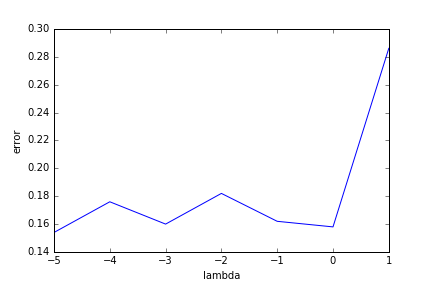
\includegraphics[width=\linewidth]{img66.png}
  \caption{Lambda range giving the minimal percent error}
  \label{fig:66}
\end{figure}

\begin{lstlisting}
Lambda = np.linspace(0,1,10)
errors = []
for i in range(len(Lambda)):
    w = pegasos_svm_change(X_train, y_train, Lambda=Lambda[i], num_iter=20)
    errors.append(percent_error(w, X_valid, y_valid))
    print(Lambda[i], percent_error(w, X_valid, y_valid))

plt.plot(Lambda, errors)
plt.xlabel("lambda")
plt.ylabel("error")
plt.savefig('/Users/twff/Downloads/machine_learning/hw/hw3-sentiment/img66b')
\end{lstlisting}

\begin{figure}
  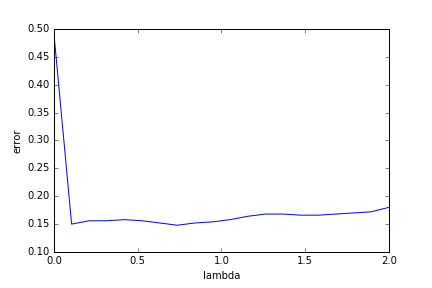
\includegraphics[width=\linewidth]{img66b.png}
  \caption{Lambda giving the minimal percent error after zooming in}
  \label{fig:66b}
\end{figure}

From the images shown, we can get when $\lambda = 0.1$, we get minimal percent error, which is 0.15.

\pagebreak
\item {[}Optional{]} Recall that the ``score'' is the value of the prediction
$f(x)=w^{T}x$. We like to think that the magnitude of the score represents
the confidence of the prediction. This is something we can directly
verify or refute. Break the predictions into groups based on the score
(you can play with the size of the groups to get a result you think
is informative). For each group, examine the percentage error. You
can make a table or graph. Summarize the results. Is there a correlation
between higher magnitude scores and accuracy?
\pagebreak
\item {[}Optional{]} Our objective is not differentiable when $y_{i}w^{T}x_{i}=1$.
Investigate how often and when we have $y_{i}w^{T}x_{i}=1$ (or perhaps
within a small distance of $1$ \textendash{} this is for you to explore)
. Describe your findings. If we didn't know about subgradients, one
might suggest just skipping the update when $yw^{T}x_{i}=1$. Does
this seem reasonable? 
\end{enumerate}

\pagebreak
\section{Error Analysis}
%%%%%%%%%%%%%%%%%%%%%%7%%%%%%%%%%%%%%%%%%%%%%%%%%%%%%%
The natural language processing domain is particularly nice in that
often one can often interpret why a model has performed well or poorly
on a specific example, and sometimes it is not very difficult to come
up with ideas for new features that might help fix a problem. The
first step in this process is to look closely at the errors that our
model makes.
\begin{enumerate}
\item Choose some examples that the model got wrong. List the features that
contributed most heavily to the descision (e.g. rank them by $\left|w_{i}x_{i}\right|$),
along with $x_{i},w_{i},xw_{i}$. Do you understand why the model
was incorrect? Can you think of a new feature that might be able to
fix the issue? Include a short analysis for at least 2 incorrect examples.%%%%%%%%%%%7.1%%%%%%%%%%%%

{\bfseries Answer 7.1}

First of all, we list the features that contributed most heavily to the decision.

\begin{lstlisting}
w_wrong = {}
for k,v in w.items():
    if abs(v)>=0.01:
        w_wrong[k] = w.get(k, 0) + v
        
w_high = pd.DataFrame(w_wrong,index=range(len(w_wrong))).T
w_high = w_high[0]
w_high
\end{lstlisting}

The results are shown as follows:
\begin{lstlisting}
also     0.041859
bad     -0.066707
best     0.029917
film     0.049779
great    0.029275
life     0.055275
love     0.022173
many     0.024715
movie   -0.059741
plot    -0.027611
story    0.022152
well     0.024776
world    0.028056
worst   -0.021296
\end{lstlisting}

We get {\bfseries 'also', 'bad', 'best', 'film', 'great', 'life', 'love', 'many', 'movie', 'plot', 'story', 'well', 'world', 'worst'} contribute most to the decision. 

Then we choose several examples that the model got wrong:
\begin{lstlisting}
def list_incorrect(w, X, y):
    '''
    w is the sparse weight vector
    X is the vector needed to be classified
    y is the true label
    --------------------------
    incorrect_list is the percent of the wrong classifiation
    '''
    incorrect_list = []
    weight_list = []
    N = len(X)
    index = []
    y_p = []
    y_true = []
    wx = []
    for i in range(N):
        yy = dotProduct(w, X[i]) 
        if yy > 0:
            yy = 1
        else:
            yy = -1
        
        if yy !=y[i]:
            incorrect_list.append(X[i])
            index.append(i)
            y_p.append(yy)
            y_true.append(y[i])
            wx.append(dotProduct(w, X[i]))
            
    return incorrect_list, index, y_p, y_true,wx   
 
import pandas as pd
summ = pd.DataFrame(index)
summ['incorr'] = incorrect
summ['y_predicted'] = yy
summ['y_true'] = yt
summ['w*x'] = wx
summ.to_csv('/Users/twff/Downloads/machine_learning/hw/hw3-sentiment/wronglist.csv')
\end{lstlisting}


\begin{table}[htbp]
 \caption{\label{tab:test}Example 1 (y-predict=1, y-true=-1)}
 \begin{tabular}{lcl}
 \hline
  Words & Weight & w*x\\
  \hline
   perfect& 0.0066 & 0.0132\\
  well & 0.0124 & 0.0124\\
  film & 0.0249 & 0.2241\\
  better & -0.0067 & -0.0134 \\
  interesting & -0.0024 & -0.0048\\
  lovely & 1e-5 &    0\\
  boring & -0.0083&  -0.0083\\
  \hline
 \end{tabular}
\end{table}


\begin{table}[htbp]
 \caption{\label{tab:test}Example 2 (y-predict=-1, y-true=1)}
 \begin{tabular}{lcl}
 \hline
  Words & Weight & w*x\\
  \hline
  new& 0.0055 & 0.022\\
  doesn't & -0.0039 & -0.0234\\
  sandler & -0.0013 & -0.0143\\
  robbie & 0.0001 & 0.0009\\
  wedding &  0.0008& 0.0064\\
  \hline
 \end{tabular}
\end{table}

The prediction of label is incorrect may due to several reasons. First of all, it may due to some negative reviews also include some positive words, which is sarcasm. But actually, the true meaning is negative. Secondly, in some positive reviews, there are some phases, such as 'It can't be better', in this case, 'can't' takes big negative weight, it is likely that the reviews will be predicted negative if the phase appears for many times. The same thing also happens on 'doesn't'. Finally, some positive words are identified as negative, such as 'better', 'interesting', or have low positive weight, like 'lovely', thus there are chances that some positive instances including plenty of this kind of words my be identified as negative incorrectly.

So the solution is that we can use bigram as features instead of using a gram. Furthermore, we can use n-gram features. Or whenever 'not' appears, it will combine with its following words as a new feature.

\end{enumerate}

\pagebreak
\section{Features}

For a problem like this, the features you use are far more important
than the learning model you choose. Whenever you enter a new problem
domain, one of your first orders of business is to beg, borrow, or
steal the best features you can find. This means looking at any relevant
published work and seeing what they've used. Maybe it means asking
a colleague what features they use. But eventually you'll need to
engineer new features that help in your particular situation. To get
ideas for this dataset, you might check the discussion board on this
\href{https://www.kaggle.com/c/sentiment-analysis-on-movie-reviews}{Kaggle competition},
which is using a very similar dataset. There are also a very large
number of academic research papers on sentiment analysis that you
can look at for ideas.
\begin{enumerate}
\item Based on your error analysis, or on some idea you have, construct
a new feature (or group of features) that you hope will improve your
test performance. Describe the features and what kind of improvement
they give. At this point, it's important to consider the standard
errors $\sqrt{p(1-p)/n}$ (where $p$ is the proportion of the test
examples you got correct, and $n$ is the size of the test set) on
your performance estimates, to know whether the improvement is statistically
significant. %%%%%%%%%%%%%%%%%%%%%%%8.1%%%%%%%%%%%%%%%%%%%%%%%%%%%%%

{\bfseries Answer 8.1}
In Biagram features:

I am going to use bigram as feature instead of a single word, that is to make every pair of consecutive words a feature.

The code list as below:

\begin{lstlisting}
def bag_of_words_bigram(words):
    '''
    words is a list of words
    -------------------
    count sparse bag of words representation.
    '''
    stop = set(stopwords.words('english'))
    words_stopfree = [w for w in words if w not in stop]
    count = Counter(words_stopfree[:-1])
    label = words[-1][1]
    return count, label
    
Xb_train  = []
yb_train = []
bigram_list = []
i=0
j=0
while i < len(training_data)-1:
    bigram_list = []
    j= 0
    i += 1
    while j < len(training_data[i])-1:
        bigram_list.append((training_data[i][j],training_data[i][j+1]))
        j += 1
    
    words, label = bag_of_words_bigram(bigram_list)
    Xb_train.append(words)
    yb_train.append(label)

Xb_valid  = []
yb_valid = []
bigram_data_test = []
i=0
while i < len(validation_data)-1:
    bigram_list = []
    j= 0
    i += 1
    while j < len(validation_data[i])-1:
        bigram_list.append((validation_data[i][j],validation_data[i][j+1]))
        j += 1
    
    words, label = bag_of_words(bigram_list)
    Xb_valid.append(words)
    yb_valid.append(label)
    
    
n = len(Xb_valid)
w = pegasos_svm_change(Xb_train, yb_train, Lambda=0.1, num_iter=20)
error = percent_error(w, Xb_valid, yb_valid)
std_error = ((1-error)*error)/n
       
\end{lstlisting}

So that the single words are turned to be bigram
\begin{lstlisting}
          ('ben', 'kingsley'): 3,
          ('ben', "kingsley's"): 1,
          ('beyond', 'an'): 1,
          ('bird', 'uses'): 1,
          ('boss', 'teddy'): 1,
          ('boulder', 'that'): 1,
          ('break', 'into'): 1,
          ('british', 'crime'): 1,
          ('british', 'gangster'): 1,
          ('buddy', 'and'): 1,
\end{lstlisting}

And the std error computed is 0.017852406801892162 in bigram examples, while in single word example, it is 0.015880554146502572, so we can conclude from the standard error that the new features is not statistically significant.


\item {[}Optional{]} Try to get the best performance possible by generating
lots of new features, changing the pre-processing, or any other method
you want, so long as you are using the same core SVM model. Describe
what you tried, and how much improvement each thing brought to the
model. To get you thinking on features, here are some basic ideas
of varying quality: 1) how many words are in the review? 2) How many
``negative'' words are there? (You'd have to construct or find a
list of negative words.) 3) Word n-gram features: Instead of single-word
features, you can make every pair of consecutive words a feature.
4) Character n-gram features: Ignore word boundaries and make every
sequence of n characters into a feature (this will be a lot). 5) Adding
an extra feature whenever a word is preceded by ``not''. For example
``not amazing'' becomes its own feature. 6) Do we really need to
eliminate those funny characters in the data loading phase? Might
there be useful signal there? 7) Use tf-idf instead of raw word counts.
The tf-idf is calculated as 
\begin{equation}
\mbox{tfidf}(f_{i})=\frac{FF_{i}}{\log(DF_{i})}
\end{equation}
where $FF_{i}$ is the feature frequency of feature $f_{i}$ and $DF_{i}$
is the number of document containing $f_{i}$. In this way we increase
the weight of rare words. Sometimes this scheme helps, sometimes it
makes things worse. You could try using both! {[}Extra credit points
will be awarded in proportion to how much improvement you achieve.{]}

{\bfseries Answer 8.2}
The code list as below:

\begin{lstlisting}
def bag_of_words_bigram(words):
    '''
    words is a list of words
    -------------------
    count sparse bag of words representation.
    '''
    stop = set(stopwords.words('english'))
    words_stopfree = [w for w in words if w not in stop]
    count = Counter(words_stopfree[:-1])
    label = words[-1][1]
    return count, label
    
Xb_train  = []
yb_train = []
bigram_list = []
i=0
j=0
while i < len(training_data)-1:
    bigram_list = []
    j= 0
    i += 1
    while j < len(training_data[i])-1:
        bigram_list.append((training_data[i][j],training_data[i][j+1]))
        j += 1
    
    words, label = bag_of_words_bigram(bigram_list)
    Xb_train.append(words)
    yb_train.append(label)

Xb_valid  = []
yb_valid = []
bigram_data_test = []
i=0
while i < len(validation_data)-1:
    bigram_list = []
    j= 0
    i += 1
    while j < len(validation_data[i])-1:
        bigram_list.append((validation_data[i][j],validation_data[i][j+1]))
        j += 1
    
    words, label = bag_of_words(bigram_list)
    Xb_valid.append(words)
    yb_valid.append(label)
    
    
n = len(Xb_valid)
w = pegasos_svm_change(Xb_train, yb_train, Lambda=0.1, num_iter=20)
error = percent_error(w, Xb_valid, yb_valid)
std_error = ((1-error)*error)/n
       
\end{lstlisting}

So that the single words are turned to be bigram
\begin{lstlisting}
          ('ben', 'kingsley'): 3,
          ('ben', "kingsley's"): 1,
          ('beyond', 'an'): 1,
          ('bird', 'uses'): 1,
          ('boss', 'teddy'): 1,
          ('boulder', 'that'): 1,
          ('break', 'into'): 1,
          ('british', 'crime'): 1,
          ('british', 'gangster'): 1,
          ('buddy', 'and'): 1,
\end{lstlisting}

And the std error computed is 0.017852406801892162 in bigram examples, while in single word example, it is 0.015880554146502572, so we can conclude from the standard error that the new features is not statistically significant.

In other cases:
\begin{table}[htbp]
 \caption{\label{tab:test}Example 1 (y-predict=1, y-true=-1)}
 \begin{tabular}{lcl}
 \hline
  methods& std error & w*x\\
  \hline
   words number& 0.01733 \\
  negative words & 0.01746\\
  bigrams & 0.015880\\
  not & 0.01955 \\
  tfidf & 0.01832 \\
  \hline
 \end{tabular}
\end{table}
\end{enumerate}

\end{document}
